\documentclass{standalone}
\usepackage{mintikz}

\begin{document}
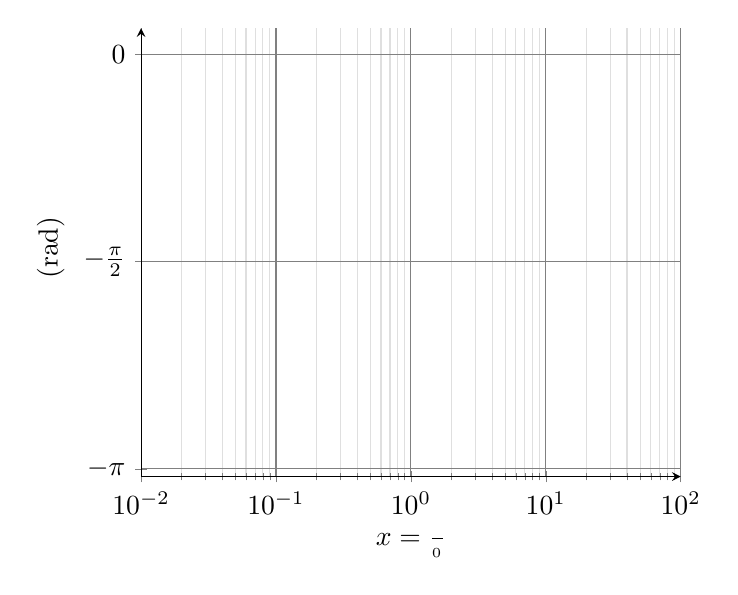
\begin{tikzpicture}[]
	\begin{semilogxaxis}[
			xmin=1e-2, xmax=1e2,
			ymin=-3.2, ymax=0.2,
			xlabel={$x=\DS\frac{\w}{\w_0}$}, ylabel=$\f$ (rad),
			ytick={0, -1.57079, -3.1415},
			yticklabels={0, $\DS-\frac{\pi}{2}$, $-\pi$},
			% extra y ticks={0.78539, 1.57079},
			% extra y tick labels={$\DS\frac{\pi}{4}$, $\DS\frac{\pi}{2}$},
			% extra y tick style={grid=none},
			axis lines=left,
			grid=both,
			major grid style={black!50},
			minor grid style={gray!25},
			clip=true]
		% \def\Q{5}
		% \addplot[
		% domain=1e-2:0.999, samples=500,
		% smooth, thick, red]
		% {-atan((\x/\Q)/(1-\x^2))*pi/180};
		% \addplot[
		% domain=1.0001:1e2, samples=500,
		% smooth, thick, red]
		% {-pi-atan((\x/\Q)/(1-\x^2))*pi/180};
		% \def\Q{.5}
		% \addplot[
		% domain=1e-2:0.999, samples=500,
		% smooth, thick, blue]
		% {-atan((\x/\Q)/(1-\x^2))*pi/180};
		% \addplot[
		% domain=1.0001:1e2, samples=500,
		% smooth, thick, blue]
		% {-pi-atan((\x/\Q)/(1-\x^2))*pi/180};
		% \addplot[
		% domain=1e-2:2,
		% smooth, black, dashed, thick]
		% {0};
		% \addplot[
		% domain=6e-1:1e2,
		% smooth, black, dashed, thick]
		% {-pi};
		% \node[red] at (axis cs:2,-0.5) {$Q=5$};
		% \node[blue] at (axis cs:.2,-1) {$Q=0.5$};
		% \draw[dashed, thick]
		% (axis cs:1e-2,-pi/2) -|
		% (axis cs:1e0,-3.5);
	\end{semilogxaxis}
\end{tikzpicture}
\end{document}
